\section{Contrived Worst-Case Results}

\begin{frame}{Contrived Case: Bird-BM Retains the Lowest Comparisons}
\centering
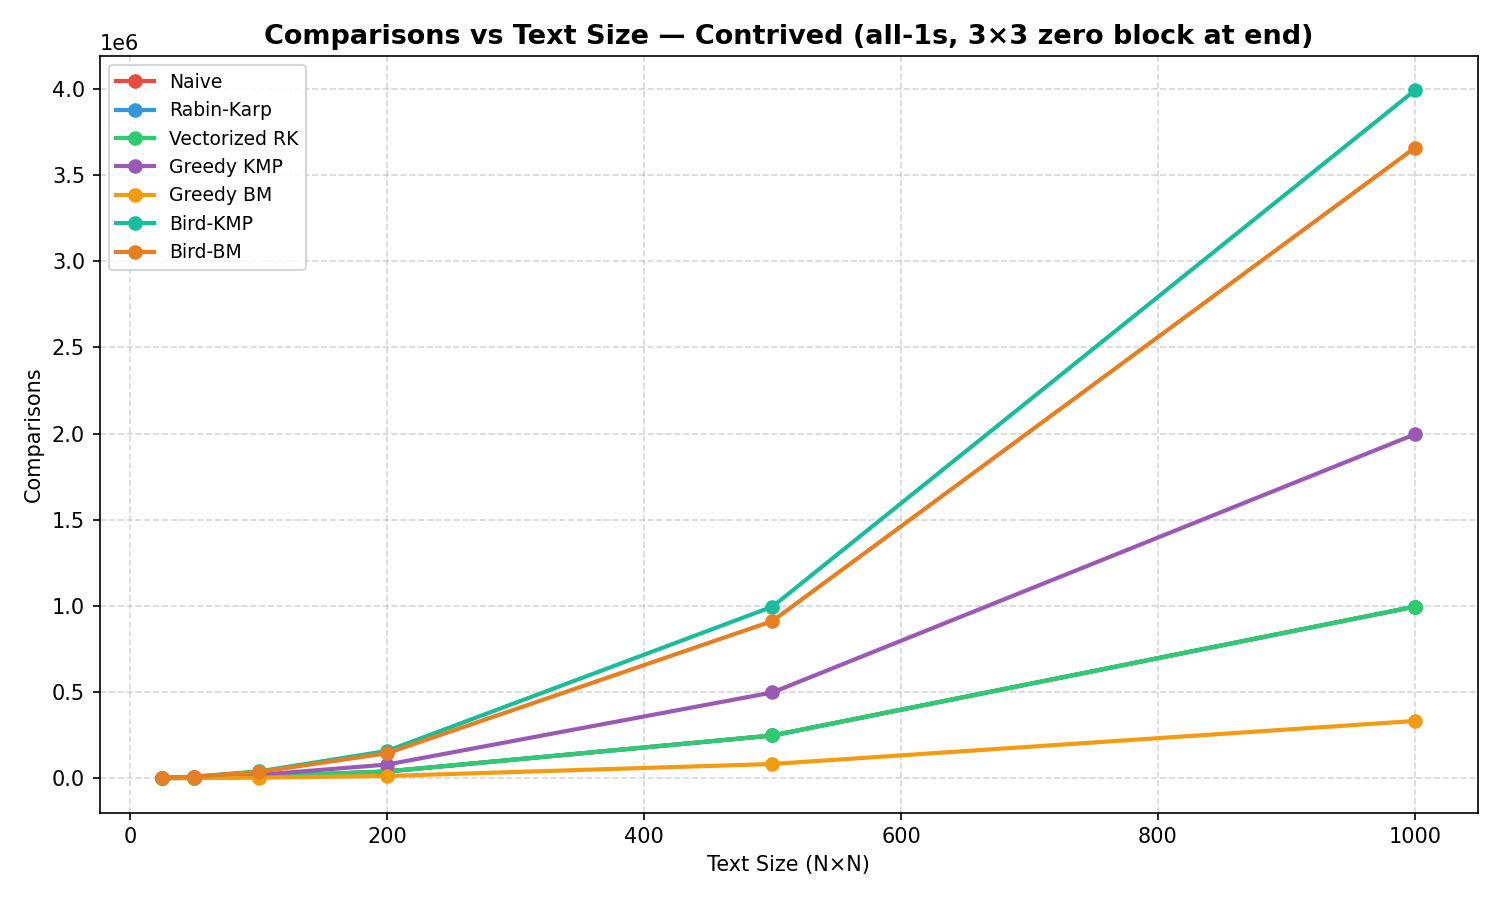
\includegraphics[width=\linewidth,height=0.50\textheight,keepaspectratio]{contrived_comparisons_vs_textsize.png}

\vspace{0.3em}
\keymsg{Best mean comparisons: \ContrivedBestCompAlgo{} (\ContrivedBestCompValue{}), while Greedy BM rises to \ContrivedCompGreedyBM{}.}
\end{frame}

\begin{frame}{Runtime Under Adversarial Placement}
\centering
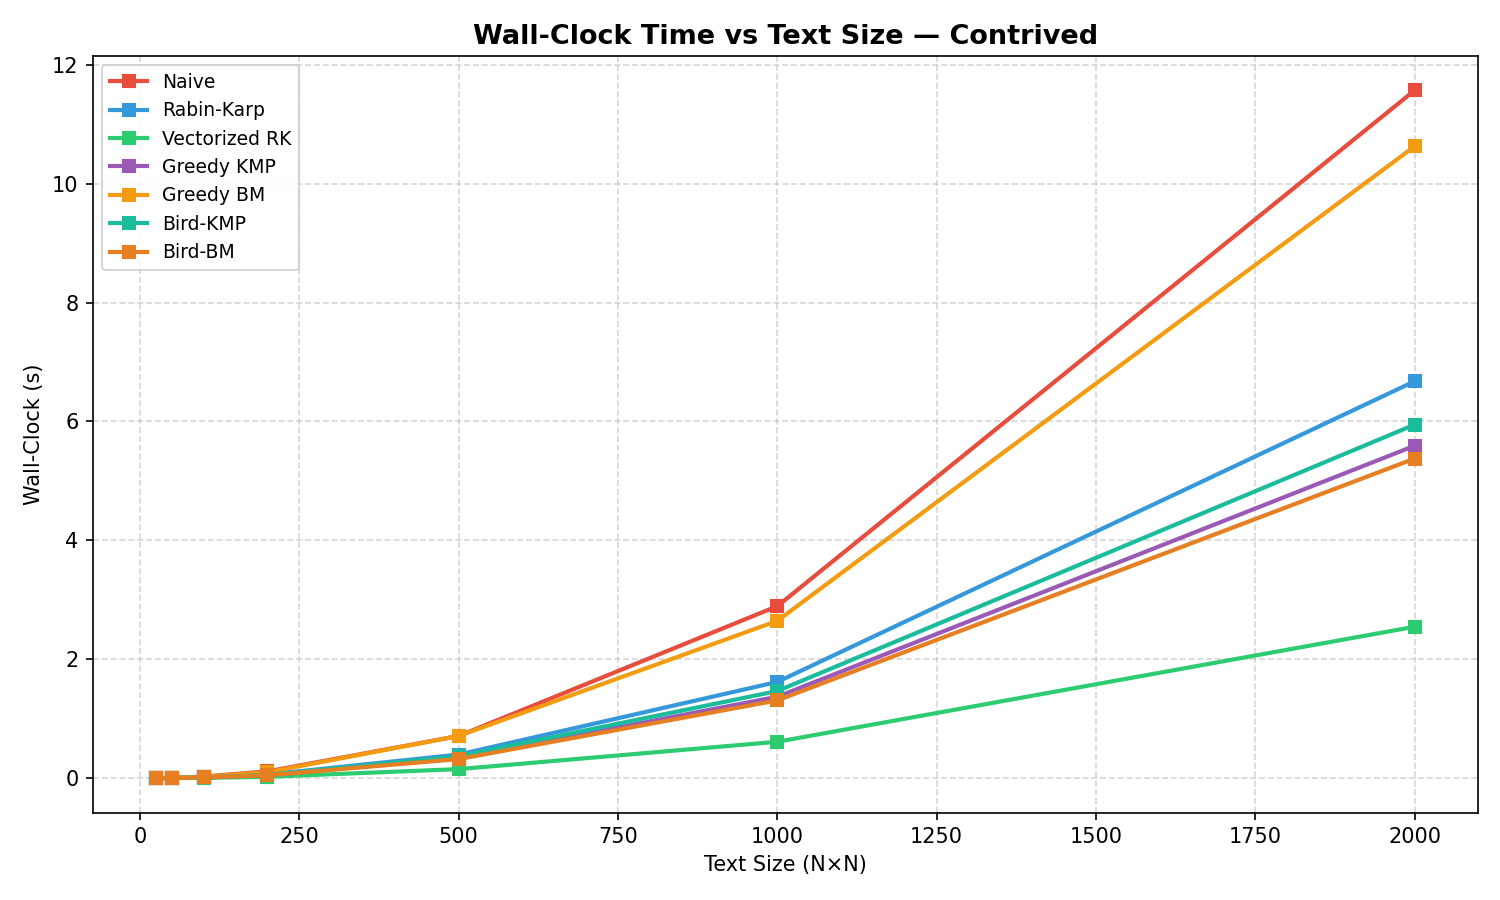
\includegraphics[width=\linewidth,height=0.50\textheight,keepaspectratio]{contrived_wallclock.png}

\vspace{0.3em}
\textbf{Winner (Runtime):} \ContrivedBestTimeAlgo{} (\ContrivedBestTimeValue{} s).
\end{frame}

\begin{frame}{Contrived Section Summary}
\small
\centering
\begin{tabular}{lrr}
\toprule
\textbf{Algorithm} & \textbf{Mean Comparisons} & \textbf{Mean Time (s)} \\
\midrule
Bird-BM & \ContrivedCompBirdBM{} & \ContrivedTimeBirdBM{} \\
Greedy BM & \ContrivedCompGreedyBM{} & \ContrivedTimeGreedyBM{} \\
Vectorized RK & \ContrivedCompVectorizedRK{} & \ContrivedTimeVectorizedRK{} \\
Naive & \ContrivedCompNaive{} & \ContrivedTimeNaive{} \\
\bottomrule
\end{tabular}

\vspace{0.5em}
\begin{block}{Interpretation}
In this contrived setup, frequent first-row triggers increase verification work; Bird-BM still keeps comparisons low, while Greedy BM degrades.
\end{block}
\end{frame}
